%----------------------------------------------------------
% DOCUMENT CLASS, PACKAGES
%----------------------------------------------------------
\documentclass[12pt, titlepage]{report}

\usepackage{pgfgantt}
\usepackage{geometry}
\usepackage{graphicx}
\usepackage{url}
\usepackage{amsmath,amssymb,amsthm}
\usepackage{rotating}
\usepackage[nottoc,numbib]{tocbibind}
\usepackage{titlesec}
\usepackage{booktabs}
\usepackage{longtable}
\usepackage{array}
\usepackage{mathtools}
\usepackage{bm}
\usepackage{epigraph}
\usepackage{amsthm}
\usepackage{todonotes}
\usepackage{dirtytalk}
\usepackage{minted}
\usepackage{neuralnetwork}


%---------------------------------------------------------
% THEOREM TYPES
%---------------------------------------------------------
\theoremstyle{definition}
\newtheorem{definition}{Definition}

\geometry{a4paper, total={170mm,257mm}, left=25mm, right=25mm, top=20mm, bottom=20mm}
\setlength{\parindent}{0em}
\setlength{\parskip}{1em}
\titleformat{\chapter}{\normalfont\huge}{\thechapter.}{20pt}{\huge}
\newcolumntype{L}[1]{>{\raggedright\arraybackslash}p{#1}}
\DeclarePairedDelimiter\ceil{\lceil}{\rceil}
\DeclarePairedDelimiter\floor{\lfloor}{\rfloor}
%----------------------------------------------------------
%----------------------------------------------------------





\begin{document}
%----------------------------------------------------------
% TITLE PAGE
%----------------------------------------------------------
\begin{titlepage}
	\newcommand{\HRule}{\rule{\linewidth}{0.5mm}}
	\center
	
	%	Headings

	\textsc{\Large Queen Mary University of London}\\[1.5cm]
	\textsc{\Large Project Report}\\[0.5cm]
	\textsc{\large Session 2017/2018}\\[0.cm]

	%	Title

	\HRule\\[0.4cm]

	{\huge\bfseries Cryptographically Secure Pseudo-Random Number Generation using Generative Adversarial Networks}\\[0.1cm]

	\HRule\\[1.5cm]

	%	Author(s)

	\begin{minipage}{0.4\textwidth}
		\begin{flushleft}
			\large
			\textit{Student}\\
			Marcello \textsc{De Bernardi}\\[0.4cm] % Your name
      \textit{Student email}\\
      m.e.debernardi@se15.qmul.ac.uk
		\end{flushleft}
	\end{minipage}
	~
	\begin{minipage}{0.4\textwidth}
		\begin{flushright}
			\large
			\textit{Supervisor}\\
			Dr. Arman \textsc{Khouzani}\\[0.4cm] % Supervisor's name
      \textit{Student phone number}\\
      07492 524132
		\end{flushright}
	\end{minipage}
  	~

	%	Date

	\vfill\vfill\vfill
	{\large\today}

	%	Logo

	\vfill\vfill
	
\includegraphics[width=0.4\textwidth]{img/qmul.jpg}\\[1cm]
	\vfill
\end{titlepage}
%----------------------------------------------------------
%----------------------------------------------------------





%----------------------------------------------------------
% ABSTRACT
%----------------------------------------------------------

\begin{abstract}
Abstract comes here!
\end{abstract}


%----------------------------------------------------------
% ACKNOWLEDGEMENTS
%----------------------------------------------------------
\renewcommand{\abstractname}{Acknowledgements}
\begin{abstract}
Acknowledgements come here!
\end{abstract}



%-------------------------------------------------
% TABLE OF CONTENTS
%-------------------------------------------------
\tableofcontents
\clearpage



%-------------------------------------------------
% INTRODUCTION
%-------------------------------------------------
\chapter{Introduction}
The availability of massive datasets during the last decade has made machine learning, and deep learning in particular, tremendously successful at solving problems throughout all areas of life \cite{russel2009artificial}. Major technology companies such as Google, Amazon, Microsoft and Facebook now all provide plug-and-play machine learning solutions as part of their cloud platforms \cite{google2018automl} \cite{amazon2018aws} \cite{microsoft2018azure}, and courses in machine learning are available at a vast number of universities as well as online. Indeed, public interest in machine learning is at an all-time high (figure \ref{figure:googletrends_dl}) \cite{forbes2016short}.

\begin{figure}
\centering
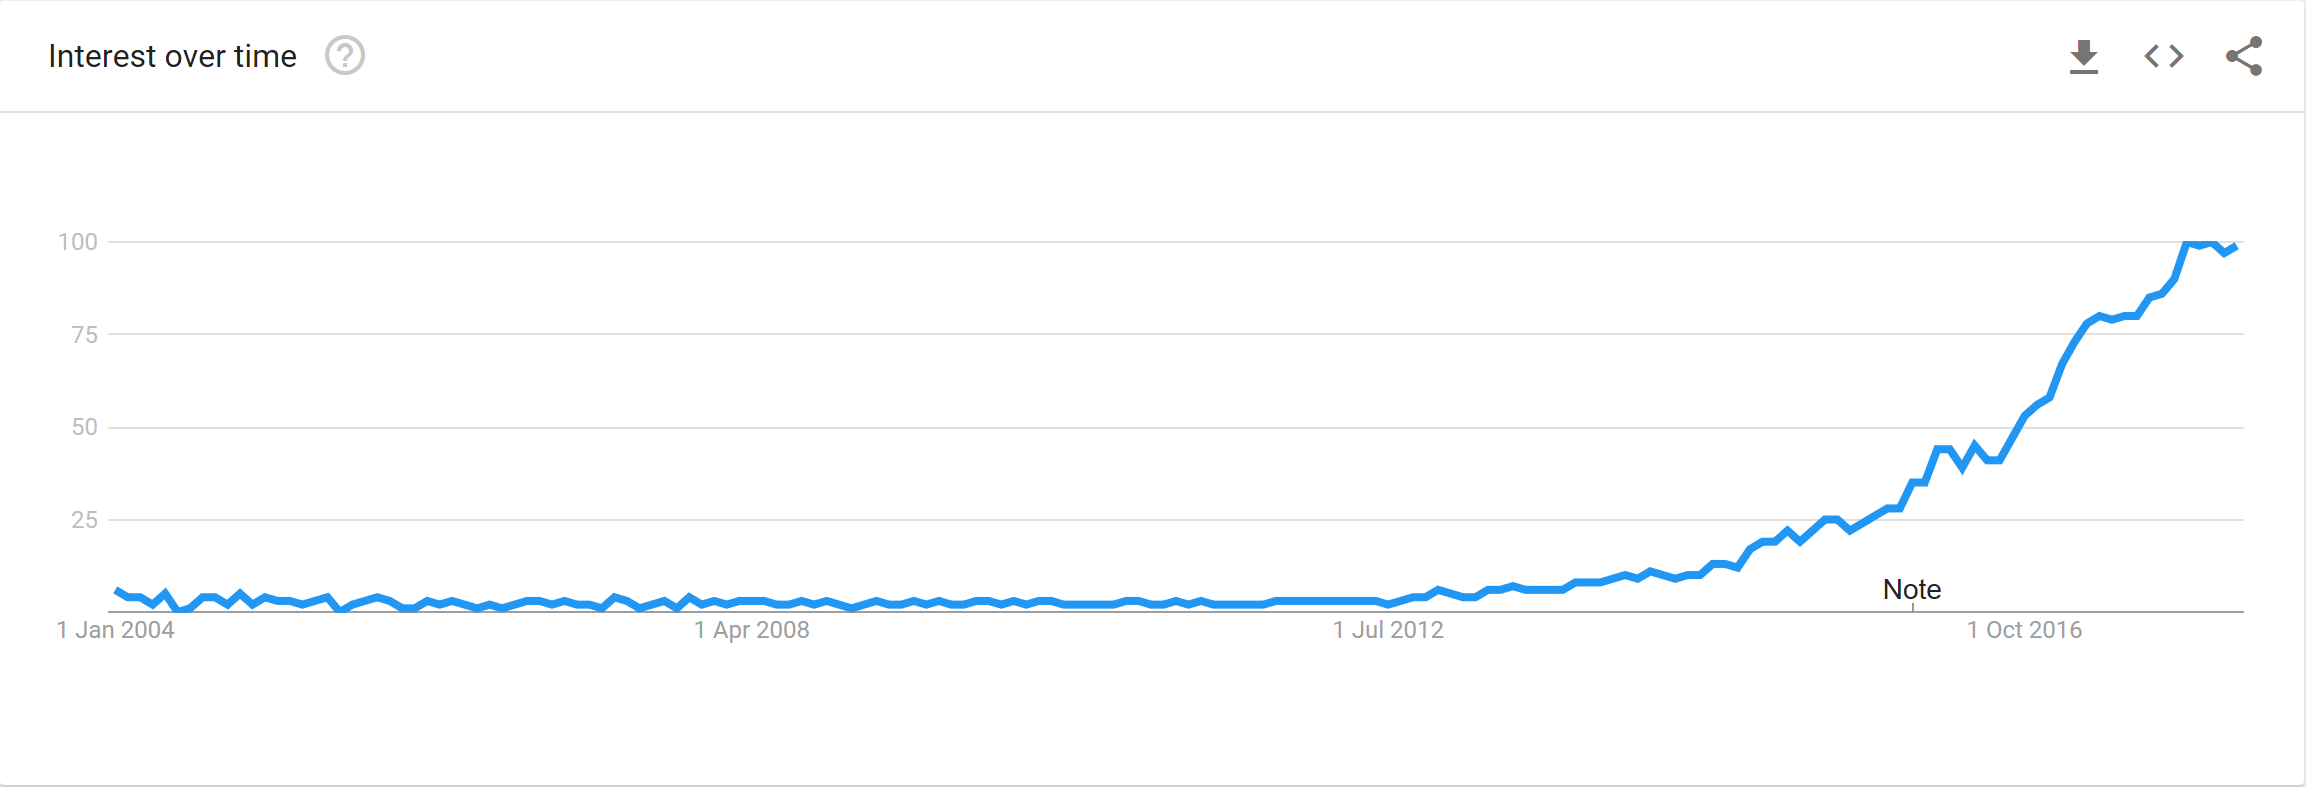
\includegraphics[width=0.95\textwidth]{img/google_trends_dl.png}\\
\caption{Search interest for "deep learning" as an example of interest in machine learning. Data source: Google Trends (www.google.com/trends) \cite{google2018trends}}
\label{figure:googletrends_dl}
\end{figure}

At the same time, 

\todo{stuff about security}


\section{Motivation}
The motivation for this work is two-fold. 

On the one hand, it presents a significant challenge from the perspective of deep learning. Neural networks have been extremely successful at learning functions to label data and perform predictions, as well as at learning how to output data mimicing a given dataset (such as images) \cite{goodfellow2014generative}. However, as outlined in section \ref{section:related_work}, attempts to produce seeming randomness in neural networks have shown somewhat poor results, and have not gained much attention.

On the other hand, this investigation is also valuable from the perspective of computer security. The ability to obtain a pseudo-random number generator "ad-hoc" by training a neural network could enable, for example, the re-initialization of a compromised PRNG into a secure state beyond what is possible by re-seeding a standard PRNG; retraining the network to a different (but satisfactory) state, while prohibitively time-consuming, would change its exact outputs in an unpredictable manner.

The undertaking of this investigation is motivated by the (unproven) conjecture that the function represented by a standard PRNG's algorithm can be approximated by a neural network of sufficient complexity.


\section{Aims}\label{subsection:aims}
The aim of this research is to determine whether \textbf{a neural network can be trained to output sequences of numbers which appear to be randomly distributed}, and, by extension, whether \textbf{such a neural network could be used as a pseudo-random number generator in a cryptographic context}.

In order to provide a conclusion for this research question, this investigation has entailed a \textbf{review of existing literature}, the design and development of a \textbf{prototype machine learning model}, \textbf{training of the model} on an HPC cluster, and finally \textbf{evaluation of the model} to determine whether training successfully resulted in a model capable of producing pseudo-random number sequences.



\section{Report Structure}
The report is structured as outlined below, with additional appendices at the end of the document.

Section \ref{chapter:background} outlines the \textbf{theoretical background} required to understand this research, as well as a literature review to capture the current state of the art in the field. The subsections are written as cohesive, self-contained units, allowing the reader to skip subsections they are already familiar with.

Section \ref{chapter:design} presents a \textbf{detailed view of the system} developed as part of this research, both at a conceptual level as well as in code. Each subsection deals with a component of the system.

Section \ref{chapter:experiments} reports the \textbf{experiments} carried out on the implementation, including the full experimental setup as well each experiment's results. These results are then analyzed.

Finally, section \ref{chapter:conclusion} makes a \textbf{conclusion} on the central research question on the basis of the results.




%----------------------------------------------------------
% BACKGROUND
%----------------------------------------------------------
\chapter{Background}\label{chapter:background}
\epigraph{Any one who considers arithmetical methods of producing random digits is, of course, in a state of sin.}{John Von Neumann, 1951}

This work lies at the intersection of machine learning and computer security. In particular, by exploring the applications of neural networks to computer security, it falls into the field of neural cryptography \cite{klimov2002analysis}. This section provides an overview of the required background to pseudo-random number generation, including definitions of random number sequences and guidelines on how to evaluate them. It also covers the basics of artificial neural networks before moving to the specific neural network techniques used in this work. Lastly, an overview of the most relevant literature is provided.

\section{Random Numbers Sequences and Generators}
Of primary concern to this research are the nature of random number sequences, and the means by which such sequences may be generated and evaluated. A consideration of the nature of randomness is sidestepped, since, as remarked by Donald Knuth, a philosophical discussion almost invariably ensues \cite[p. 2]{donald1998art}. Instead, a pragmatic set of definitions for the key terminology is provided.

\subsection{Random Bits, Random Numbers, and Entropy}
The definitions of random numbers rely on ideas from basic probability theory, such as sample spaces, random variables, and probability distribution functions. As this work deals with sequences of numbers that are to be encoded in a fixed-digit format, whatever that format may be, it shall be implicit that all discussions of sample spaces and random variables refer to discrete sets and discrete probability distribution functions.

\begin{definition}
A \textbf{random number} $x$ is a numeric value selected at random from an equiprobable sample space $\Omega$. That is, the probability $\mathbb{P}(x)$ of the value being chosen from $\Omega$ is equal to that of all other possible values in $\Omega$ \cite[p. 7]{barker2007recommendation} \cite[s. 1.1.1]{rukhin2001statistical}. It follows that a discrete random variable $X$ defined as the outcome of a selection from $\Omega$ has the \textbf{discrete uniform distribution}.
\end{definition}

\begin{definition}
A \textbf{random bit} $b$ is a special case of a random number, such that the equiprobable sample space is $\Omega = \{0, 1\}$ \cite[s. 1.1.1]{rukhin2001statistical}.
\end{definition}

\begin{definition}
As defined by Barker et al and Rukhin et al, a \textbf{random sequence} $s = (x_0, x_1, ..., x_n)$ is a sequence of random values $x_i$ resulting from sequential independent selections. In other words, a random sequence is a sequence of random numbers such that the result of any previous selection within the sequence does not affect future selections within the sequence. The random sequence has the same probability of being sampled as all other sequences of the same length \cite[p. 7]{barker2007recommendation} \cite[s. 1.1.1]{rukhin2001statistical}.
\end{definition}

Every binary sequence represents, in some particular encoding scheme, a unique numerical value. For example, the binary sequence $101$ is the unsigned integer representation of the number $5$. This results in an equivalence between random binary sequences and random numbers, in that the probability of randomly sampling any particular binary sequence of length $l$ from the set $\{0, 1\}$ is the same as that of selecting any particular number from the set of $2^l$ numbers representable in the binary encoding scheme used. As observed by Menezes et al, we can therefore regard the task of producing a random number as equivalent to the task of producing a random binary sequence of the appropriate length \cite[p. 170]{menezes1996handbook}.

Lastly, to quantify the randomness of a number sequence, the information theory concept of entropy is introduced. We view entropy as a measure of the uncertainty of a random variable, and define it as follows.

\begin{definition}
Let $X$ be a discrete random variable over a sample space $\Omega$ with a probability distribution function $p(x)=\mathbb{P}\{X=x\}, x\in\Omega$.  The \textbf{entropy} $H(X)$ of the discrete random variable $X$ is defined as
\begin{gather}\label{eq:entropy}
H(X) = -\sum_{x\in\Omega} p(x) \lg p(x)
\end{gather}
Entropy is measured in bits, and the base of the logarithm in the defining equation is $2$ \cite[p. 12-13]{cover2012elements}.
\end{definition}

The following intuitive formulation of entropy was given by Ferguson et al. Entropy can thought of as the average number of bits one would need in order to specify some (partially) unknown value under an ideal compression scheme. It is a subjective quantity, in the sense that it depends on the amount of knowledge available about the value of interest. The entropy of an arbitrary number is different for an observer that knows the number, and for one that only knows the value is one of $2^32$ possible values. The more uncertain we are about the value, the higher the entropy \cite[p. 137]{ferguson2010cryptography}.



\subsection{Applications of Random Numbers}
Random numbers have several important applications in computing, primarily in cryptography, where many algorithms make use of randomness, \cite[p. 137]{ ferguson2010cryptography} and in science, where simulations of random processes are frequently used\cite{deng2017developments}. A few important examples are considered here.

The \textbf{RSA (Rivest-Shamir-Adleman) algorithm}, as explained by Anderson [p. 171]\cite{anderson2010security}, is the most commonly used algorithm for performing public-key encryption and digital signatures. The RSA algorithm relies on two randomly chosen large prime numbers $p$ and $q$, which act as the private keys used by the two communicating parties. As these values must be kept secret from any third parties, they need to be selected randomly in such a manner than an attacker cannot predict them.

The \textbf{HTTP digest access authentication protocol} \todo{find RFC}

\textbf{Monte Carlo methods} \todo{MCTS}



\subsection{Random Number Generators}
In order to obtain sequences of random numbers for use in applications such as those mentioned above, random number generators are used.

\textbf{Definition}. Menezes et all \cite{menezes1996handbook} define a \textbf{random number generator} as a software or hardware system that outputs random number (or bit) sequences. Key components of such a system are the \textbf{entropy source}, which gives rise to the randomness in the output, and the \textbf{entropy distillation} process, which is a function applied to the inputs to improve the quality of the output sequence.

According to Ferguson et al and Menezes et al, entropy sources are commonly implemented in software, hardware, or both. Examples of entropy sources that are harnessed by software means include the timings of keystrokes on a computer user's keyboard, the current value of the system clock, the content of an I/O buffer, or any other measurable quantity in a computer system that is conjectured to exhibit random behavior. This conjecture does not always hold; for example, the time elapsed between keystrokes may not be accurately described by a uniform distribution, as an experienced typist may manage to keep their typing rate remarkably constant (with fluctuations on the order of several milliseconds). Care has to be taken to not overestimate the amount of entropy that can be derived from a source \cite[p. 138-139]{ferguson2010cryptography} \cite[p. 171-172]{menezes1996handbook}.

Ferguson et al and Menezes et al also discuss hardware entropy sources. These rely on physical processes that behave randomly. Commonly cited examples are emission times of particles during radioactive decay or thermal noise in a resistor. While there are very many such processes (in particular in the "quantum realm"), physically based entropy sources are not necessarily secure either. Even if a process behaves randomly, the outputs may nonetheless be biased or correlated, possibly due to manipulation on the attacker's part. Furthermore, an attacker may be able to observe the physical entropy source, meaning that while the data may still be random, it will have no entropy from the adversary's perspective \cite[p. 138-139]{ferguson2010cryptography} \cite[p. 172]{menezes1996handbook}.

According to Ferguson, Schneier, and Kohno, there are several problems related to the practical use of truly random numbers. Real random data may not always be available, and even if available it is nonetheless always limited in quantity. For example, for an RNG relying on a user's keystrokes, it may be the case that the user has not been typing sufficiently. Waiting for more real random data to be acquired in order to receive random numbers is not a viable option for a number of applications \cite[p. 139]{ferguson2010cryptography}. Furthermore, it is difficult to ascertain how much entropy one is really getting from the source, not to mention that the source, in particular if implemented in hardware, may fail unexpectedly and become predictable \cite{ferguson2010cryptography}.



\subsection{Pseudo-Random Number Generators}
A solution to many of the problems inherent to the use of truly random number generators is to use a pseudo-random number generator \cite[p. 140]{ferguson2010cryptography}.

\begin{definition}
 A \textbf{pseudo-random number generator} is a deterministic algorithm that outputs number sequences that are statistically indistinguishable from random sequences \cite{menezes1996handbook}. A PRNG has an internal state $S$, which is secret \cite{kelsey1998cryptanalytic}, and takes an input value, referred to as the \textbf{seed}, which is randomly selected as well as unknown \cite[s. 1.1.4]{rukhin2001statistical}. The outputs of the PRNG are a function of the seed and the internal state \cite{kelsey1998cryptanalytic} \cite[s 1.1.4]{rukhin2001statistical}, and so we can formalize a PRNG as a function $f(s, S)$, where $s$ is the input seed and $S$ is the internal state (see figure \ref{figure:prng_high_level}).
\end{definition}

\begin{figure}
\centering
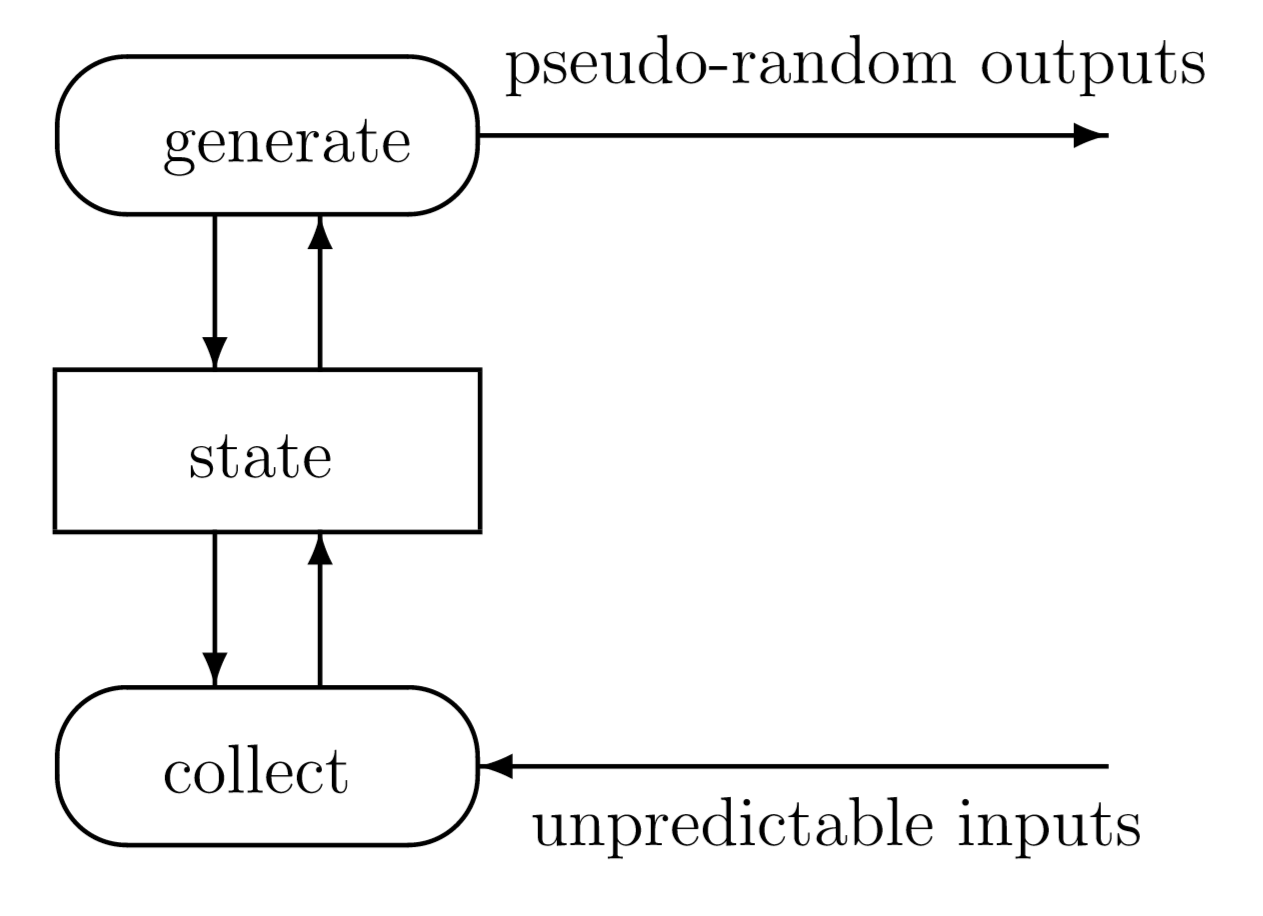
\includegraphics[width=0.65\textwidth]{img/prng_high_level.png}\\
\caption{A high-level view of the operation of a PRNG \cite{kelsey1998cryptanalytic}.}
\label{figure:prng_high_level}
\end{figure}
	


\subsection{Cryptographic Randomness Requirements}\label{subsection:crypto_requirements}
TODO: a reasonable list of the security requirements of a PRNG in order to be termed a CSPRNG. I have multiple sources on this, but no one good source.



\subsection{Testing Pseudo-Random Sequences}\label{subsection:testing_prngs}
The \textbf{National Institute of Standards and Technology}, part of the U.S. Department of Commerce, sets out guidelines for the testing of RNGs and PRNGs in its publication 800-22, \textit{A Statistical Test Suite for Random and Psuedorandom Number Generators for Cryptographic Applications}, by Rukhin et al. This work refers to revision 1a of the publication.

Rukhin et all point out that, since the properties of random sequences can be described in probabilistic terms, their degree of ``randomness" can be evaluated by various statistical tests, as the likely outcome of such a test is known a priori. These tests search for particular patterns in sequences which would indicate non-randomness. No set of statistical tests can be considered complete, as there is an infinite number of tests \cite[p. 1-2]{rukhin2001statistical}.

Also according to Rukhin et al, statistical tests are formulated to test for the \textbf{null hypothesis} $H_0$ that the sequence under review is random. Each test either accepts the null hypothesis, or rejects the null hypothesis and accepts the \textbf{alternative hypothesis} $H_a$ that the sequence is not random. Under the assumption of randomness, any statistical metric has a theoretical reference distribution which can be determined mathematically \cite[p. 1.3]{rukhin2001statistical}. For example, for a random sequence, the ratio of 1s to 0s has the probability distribution shown in figure \ref{figure:distribution}.

\begin{figure}
\centering
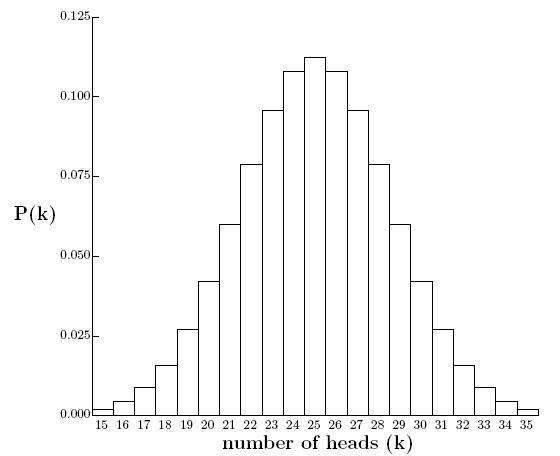
\includegraphics[width=0.7\textwidth]{img/distribution.jpg}\\
\caption{The probability distribution of a random variable representing the number of heads in a repeated fair coin-tossing experiment, which is equivalent to repeated random sampling from ${0, 1}$. Image from \cite{terr2009math}.}
\label{figure:distribution}
\end{figure}
	
From such a distribution, a \textbf{critical value} is determined. This value acts as a threshold to which the value of a metric computed on a sequence is compared. If the computed value exceeds the critical value, we assert that the test rejects the null hypothesis. Intuitively, the idea is that we consider a value above the critical value to be so unlikely to occur (though not impossible) under the assumption of randomness, that we can confidently reject the randomness hypothesis \cite[p. 1.3]{rukhin2001statistical}.

The NIST Test Suite is the accepted standard for testing random and pseudo-random bit generators \cite{lavasani2009practical}. It consists of a battery of statistical tests performed on file containing large binary sequences. Each test in the suite either accepts or rejects the null hypothesis \cite{rukhin2001statistical}. The NIST suite was found to be used throughout the majority of papers on PRNGs reviewed at the start of this investigation.



\section{Artificial Neural Networks}
This investigation approaches the problem of generating pseudo-random number sequences using neural networks. An introduction to neural networks, as well as some of the specific neural network architectures used, is given in this section.



\subsection{Introduction to Neural Networks}\label{subsection:neural_intro}
From section 18.7 of Russel and Norvig's \textit{Artificial Intelligence: A Modern Approach}, the following definition of an artificial neural network can be constructed.

\begin{definition}
An \textbf{artificial neural network} is a directed graph composed of \textbf{units} or \textbf{neurons} connected by directed \textbf{links}. Each unit computes an arbitrary \textbf{activation function} $g$ over the weighted sum of the unit's inputs. A link from unit $i$ to a unit $j$ propagates the output of the activation function of $i$ from $i$ to $j$. Each such link has an associated \textbf{weight} $w_{ij}$, which is a coefficient applied to the propagated activation value \cite[p. 727-731]{russel2009artificial}.
\end{definition}

The weighted sum of the inputs to a neuron $j$ is given by
\begin{gather}\label{eq:weighted_sum}
in_j = \sum_{i=0}^{n} w_{i,j}a_i
\end{gather}
where $n$ is the number of units with a directed edge to $j$, $w_{i,j}$ is the weight of the edge from a node $i$ to the node $j$, and $a_i$ is the output value of each node $i$. Equivalently, this can be formulated as the inner product of the output vector $\bm{a_i}$ and weight vector $\bm{w_{i,j}}$. The activation of the unit is computed by applying the activation function to this sum, as given by
\begin{gather}\label{eq:activation}
a_j = g(in_j) = g\left(\sum_{i=0}^{n} w_{i,j}a_i\right)
\end{gather}
where $a_j$ is the activation of node $j$, $g$ is the activation function, and $in_j$ is the weighted sum of the inputs as given in \ref{eq:weighted_sum}.

\begin{figure}
\centering
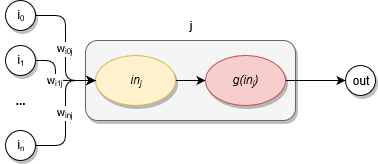
\includegraphics[width=0.7\textwidth]{img/neuron.png}\\
\caption{Schematic of the computation performed by a unit, from Russel and Norvig \cite[p.728]{russel2009artificial}. This schematic corresponds to equation \ref{eq:activation}.}
\label{figure:neural_unit}
\end{figure}

The properties of the network are determined by the topology and behavior of its units. Thus we classify networks depending on the types of units they contain, as well as on the topology of their connections \cite[p. 729]{russel2009artificial}. 

An alternative definition of neural networks, also from Russel and Norvig, can be expressed in more purely mathematical terms. We can view a neural network as  a representation of a highly non-linear vector function $\bm{f}_{\bm{w}}(\bm{x})$ parameterized by its weights $\bm{w}$ \cite{russel2009artificial}. The function $\bm{f}$ represented by the network as a whole is the composition of $i$ functions $\bm{f}^(i)$ arranged into a sequence \cite{goodfellow2016deep}, which can be expressed as
 \begin{gather}\label{eq:neural_net_composition}
 \bm{f_w}(\bm{x}) = \bm{f_{w_{i - 1}}}^{(i - 1)}(\bm{f_{w_{i - 2}}}^{(i - 2)}(... \bm{f_{w_0}}^{(0)}(\bm{x}) ...))
\end{gather}

where $\bm{w_i}$ is the output weight vector for the units collectively computing the function $\bm{f_{w_i}}^{(i)}$ \cite{goodfellow2016deep}.

According to Russel and Norvig, a neural network of sufficient size can represent any continuous function to an arbitrary degree of accuracy, and, under certain conditions, can even represent discontinuous functions. However, difficulties arise in determining, for any particular network architecture, the set of functions it can represent \cite{russel2009artificial}. This property of neural networks is at the heart of this investigation's hypothesis.



\subsection{Learning in Neural Networks}
The task of training an artificial neural network entails finding a combination of weight parameters $\bm{w}$ which results in the network's function $h(x)$ approximating the desired function $f(x)$ as closely as possible \cite[p. 718]{russel2009artificial}. The most important concepts in this regard are loss functions, the gradient descent algorithm, and the backpropagation algorithm.
 
\begin{definition}
A \textbf{loss function} $L(y, y', x)$ is defined by Russel and Norvig as "the amount of utility lost' by predicting $h(x) = y'$ when the correct answer is $f(x) = y$", where $h$ is the function represented by the neural network, and $f$ is the "true" function mapping the inputs to their correct outputs. A simpler, commonly used formulation is $L(y, y')$, which is independent of the input $x$ \cite{russel2009artificial}.
\end{definition}

Intuitively, a loss function provides a quantitative assessment of how closely the neural network approximates the desired function. A good model will have low loss. Overall, learning in neural networks is an optimization problem, in which the objective is to minimize the loss function with respect to the parameters of the network \cite[Linear classification: Support Vector Machine, Softmax]{karpathy2017cs231n}.

\begin{definition}
\textbf{Gradient descent} is an optimization algorithm in which the gradient of a function is computed with respect to the function's parameters, and the parameters are modified in the opposite direction relative to the gradients, in order to minimize the output of the function on its inputs \cite{[Optimization: Stochastic Gradient Descent] karpathy2017cs231n}.
\end{definition}

Gradient descent is currently ubiquitous in the optimization of neural network loss functions. A high-level expression of gradient descent, from \cite{karpathy2017cs231n}, is as follows:

\begin{minted}{python}
  while True:
    weights_grad = evaluate_gradient(loss_fun, data, weights)
    weights += - step_size * weights_grad  # parameter update
\end{minted}

Karpathy's lecture notes on gradient descent state that an important design choice is whether to perform \textbf{batch} gradient descent, \textbf{mini-batch} gradient descent, or \textbf{online} gradient descent (known also as stochastic gradient descent). In the first case, the gradients are computed with respect to the network's parameters over the entire training dataset, performing a single gradient update. In some applications, however, the sheer size of the dataset can make this both impractical and wasteful. Thus it is very common to split the training data into "mini-batches", and perform a single gradient update for each mini-batch. In the extreme case of online gradient descent, a gradient update is performed for each input to the network. Other aspects of the gradient descent algorithm can also be tweaked to modify its behavior \cite[Optimization: Stochastic Gradient Descent]{karpathy2017cs231n}. 

\begin{definition}
\textbf{Backpropagation} is an efficient algorithm for computing the partial derivative of a function of many variables by repeated application of the chain rule of derivation \cite[Backpropagation, Intuitions]{karpathy2017cs231n}. 
\end{definition}

This investigation does not consider the details of backpropagation, as the backpropagation algorithm is a core component of all modern machine learning software libraries, and can mostly be dealt with as a black box. The significance of backpropagation to deep learning is that it enables efficiently computing the gradient of the loss function with respect to each parameter in the neural network \cite[Backpropagation, Intuitions]{karpathy2017cs231n}

These three components enable learning in neural networks: the loss function quantifies the quality of the current parameters, gradient descent is the general optimization algorithm for modifying the parameters, and backpropagation enables efficient computation of gradients, making gradient descent on large networks practically feasible \cite[Optimization: Stochastic Gradient Descent]{karpathy2017cs231n}.



\subsection{Activation Functions}
The concept of an \textbf{activation function} was briefly introduced in \ref{subsection:neural_intro}, as an arbitrary scalar function applied to the weighted sum of a unit's inputs to produce the unit's output. There are a number of standard activation functions that are commonly used. Traditionally popular activations are the \textbf{sigmoid} and \textbf{tanh} activations, although they have fallen out of favor in recent years \cite[Neural Networks Part 1: Setting up the Architecture]{karpathy2017cs231n}. An explanation can be found in appendix \ref{appendix:mathematics}. The most relevant activations to this investigation are the ReLU and LeakyReLU functions.

\begin{definition}
The \textbf{ReLU} activation, or \textbf{Rectified Linear Unit}, is a function $ReLU: \mathbb{R} \rightarrow \mathbb{R}^+$ with the following expression form:
\begin{gather}\label{eq:relu}
ReLU(x) = max(0, x)
\end{gather}
\end{definition}

The ReLU activation function has been found to work well in practice on a large number of problems, and has become very popular in the last few years. However, it is possible for a ReLU unit to have its weights updated in a way that causes them to never be updated again due to the 0 gradient for all negative inputs \cite[Neural Networks Part 1: Setting up the Architecture]{karpathy2017cs231n}.

\begin{definition}
The \textbf{leaky ReLU} activation is a function $LeakyReLU: \mathbb{R} \rightarrow \mathbb{R}$ with the following expression form:
\begin{gather}\label{eq:leakyrelu}
LeakyReLU(x) = 
\begin{cases}
    x 							 & \text{if } x\geq 0\\
    \alpha{x}             & \text{otherwise}
\end{cases}
\end{gather}
where $\alpha$ is a (small) non-zero constant \cite[Neural Networks Part 1: Setting up the Architecture]{karpathy2017cs231n}.
\end{definition}

\begin{figure}
\centering
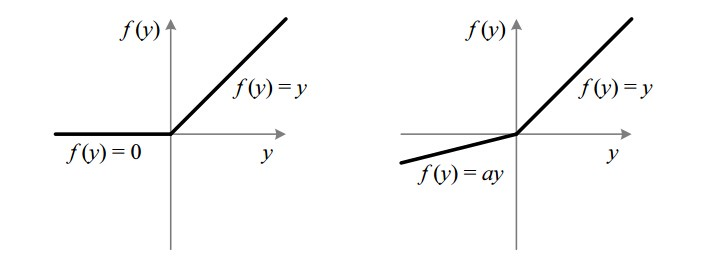
\includegraphics[width=0.7\textwidth]{img/relu.jpg}\\
\caption{Left: the ReLU function. Right: the LeakyReLU function. Image courtesy of \cite{sharma2017activation}.}
\label{figure:relu}
\end{figure}

As explained by Karpathy, the leaky ReLU eliminates the 0 gradient by assigning all negative values a small non-zero gradient. For negative inputs close to 0 the outputs of the leaky ReLU are approximately equal to the outputs of the standard ReLU function, but the units cannot "die" due to getting stuck in a flat gradient. A further variant, called \textbf{PReLU}, or \textbf{parametric leaky ReLU}, makes $\alpha$ a learnable parameter  \cite[Neural Networks Part 1: Setting up the Architecture]{karpathy2017cs231n}.



\subsection{Feed-Forward Networks}
The arguably simplest form of an artificial neural network is called a \textbf{feed-forward neural network}, or \textbf{multilayer perceptron}. Feed-forward networks are characterized by the fact that the directed graph representing them is acyclic; that is, information strictly flows from the network's input units towards its output units \cite[p. 164]{goodfellow2016deep}.

Goodfellow et al explain that feed-forward networks are typically arranged into fully connected \textbf{layers} of units, where we refer to the number of layers as the \textbf{depth} of the network. The first layer of the network is referred to as the \textbf{input layer}, within which each unit corresponds to a single scalar in the model's input vector. The last layer is referred to as the \textbf{output layer} of the network, where each unit corresponds to a scalar in the model's output vector. The number of units in the input and output layers are thus bound by the dimensionality of the input data and the dimensionality of the expected outputs. Finally, we refer to the intermediate layers as \textbf{hidden layers}, and to the number of units in the largest of these layers as the \textbf{width} of the model \cite[p. 164-165]{goodfellow2016deep}. This information is conveyed pictorially in figure \ref{figure:feedforward}.

\begin{figure}
\centering
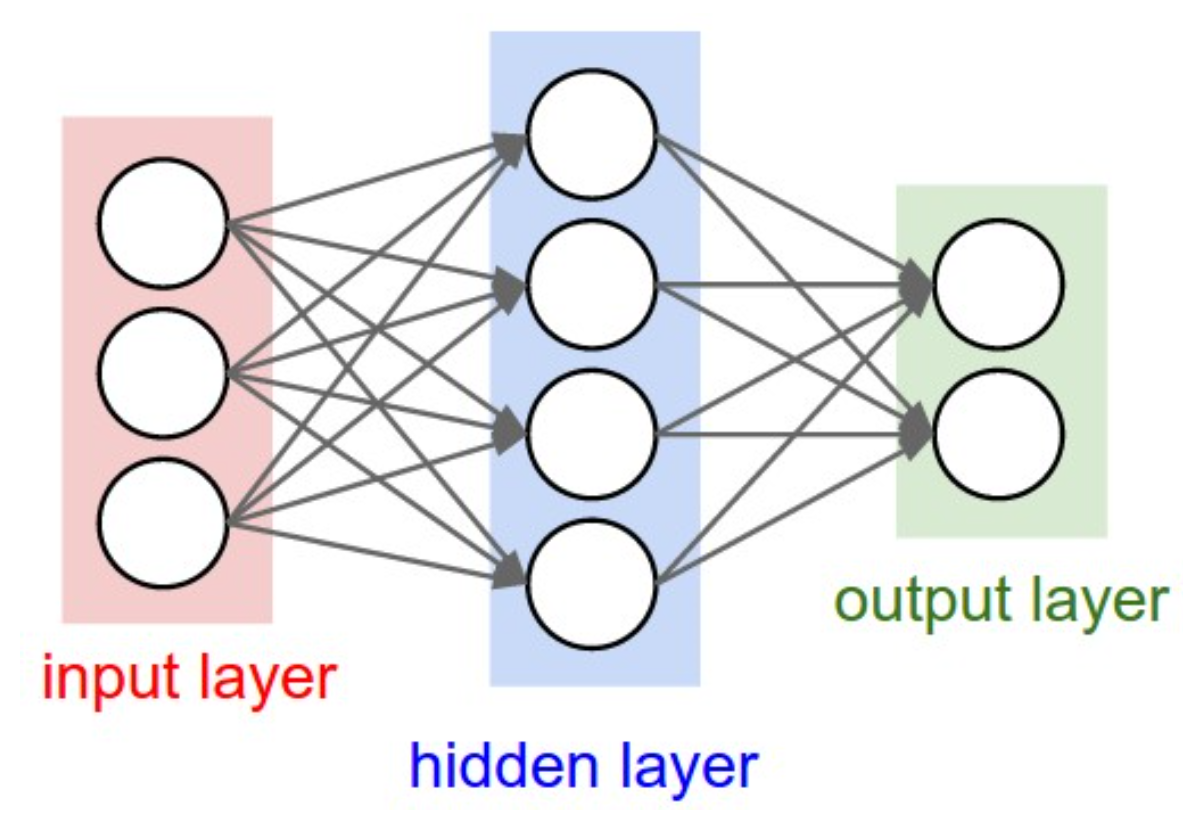
\includegraphics[width=0.7\textwidth]{img/feedforward.png}\\
\caption{Simple example of the structure of a feedforward network, from the CS231n lecture notes by Andrej Karpathy \cite[Neural Networks Part 1 : Setting up the Architecture]{karpathy2017cs231n}}.
\label{figure:feedforward}
\end{figure}

In a fully connected feed-forward network, the operation of each layer can be characterized as a simple matrix operation, whereby the input vector received from the previous layer is first transformed by element-wise application of the activation function, and then matrix-multiplied with the weight vector of the current layer \cite[p. 170-171]{goodfellow2016deep}. Thus the network as a whole is a sequence of matrix multiplications and element-wise applications of non-linearity.



\subsection{Convolutional Neural Networks}
A more specialized form of artificial neural network is the \textbf{convolutional neural network}, which is characterized by the fact that there is at least one pair of layers between which a \textbf{convolution} is performed, rather than a general matrix multiplication \cite[p. 326]{goodfellow2016deep}. A description of the convolution operation is given in appendix \ref{appendix:mathematics}. Convolutional neural networks are the state of the art for classification of signals and images \cite[p. 326]{goodfellow2016deep}.

\begin{figure}
\centering
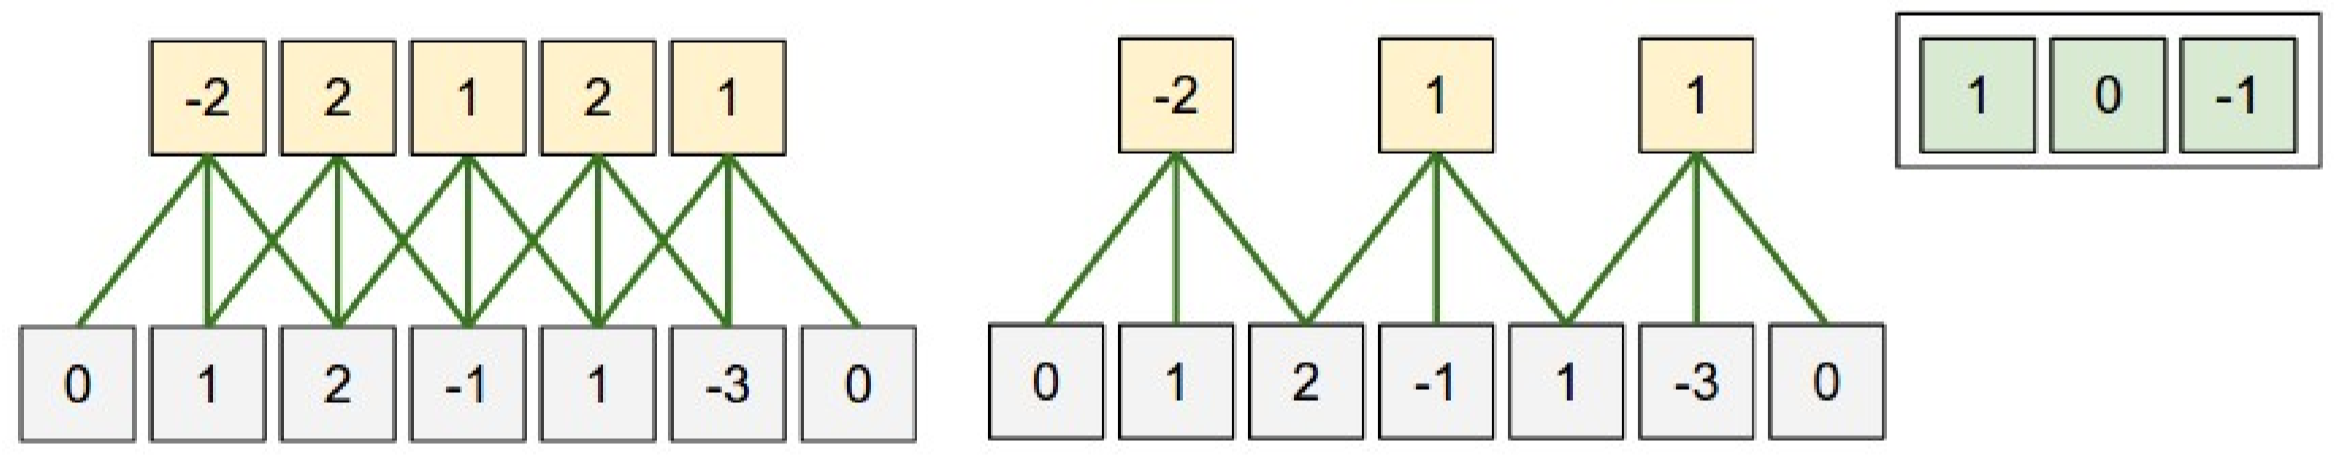
\includegraphics[width=0.85\textwidth]{img/convolution.png}\\
\caption{A representation of the connectivity between the units of a 1-dimensional input layer (white) and a single filter in a convolutional layer (yellow), with each neuron's weights in the upper right corner. In both images, each unit in the convolutional layer has a receptive field (or kernel size) of 3. The inputs have a width of 5, with zero-padding of 1. The two images demonstrate different strides for the convolutional layer (stride 1 on the left, stride 2 on the right). Image courtesy of the CS231n lecture notes by Andrej Karpathy \cite[Convolutional Neural Networks: Architectures, Convolution / Pooling Layers]{karpathy2017cs231n}.}
\label{figure:convolution1d}
\end{figure}

A convolutional layer is a collection of units, further subdivided into collections referred to as \textbf{filters}. The number of filters in the layer is referred to as the \textbf{depth} of the layer, while the dimensions of each individual filter are referred to as the \textbf{width} and \textbf{height} of the layer (for filters operating on 1-dimensional inputs only the width is of relevance). With respect to the previous layer in the network, each filter has the same connection topology \cite[Convolutional Neural Networks: Architectures, Convolution / Pooling Layers]{karpathy2017cs231n}.

Filters in a convolutional layer are not fully connected to the previous layer. Rather, each unit in the filter is connected to $F$ consecutive units in the previous layer. $F$ is referred to as the \textbf{receptive field}, or \textbf{kernel size}, of the convolutional layer. A further parameter, called the \textbf{stride} of the layer, $S$, determines the sparsity of the connections between the filters and the previous layer \cite[Convolutional Neural Networks: Architectures, Convolution / Pooling Layers]{karpathy2017cs231n}. The nature of this connectivity for a single filter is shown in figure \ref{figure:convolution1d}. The figure also demonstrates the use of zero-padding, i.e. expanding the input vector with 0s on either side in order to make it fit the convolutional layer's size requirements.

Each unit in the convolutional layer will produce larger outputs for some inputs in its receptive field than others. For example, a unit with receptive field $F = 3$ may compute a larger value for an input $[1, 1, 1]$ than an input $[0, 0, 0]$. Each unit will therefore "activate" upon finding some specific pattern (in this case a sequence of three 1s). An important optimization in convolutional layers is \textbf{parameter sharing}: each unit within the same filter shares the same weights. This optimization arises from the assumption that, if some pattern in the input is of interest at one location in the input sequence, it will be at any other location as well. Thus the parameters of every unit in each filter are trained together \cite[Convolutional Neural Networks: Architectures, Convolution / Pooling Layers]{karpathy2017cs231n}.

As a result, each filter in the layer can be seen as looking for a specific pattern in the input received from the previous layer. The depth of the convolutional layer, i.e. the number of filters, determines the number of patterns being looked for. The dimensionality of a convolutional layer's output is $d + 1$, where $d$ is the dimensionality of the output of the previous layer: with $N$ filters, the convolutional layer outputs $N$ matrices of the same size as the layer's input. Convolutional layers are usually followed by \textbf{pooling layers}, which are non-parametric layers that perform a down-sampling of the convolutional layer's outputs. This expansion along the depth-dimension, followed by down-sampling in the width and height dimensions, is shown in figure \ref{figure:conv_pooling}.

\begin{figure}
\centering
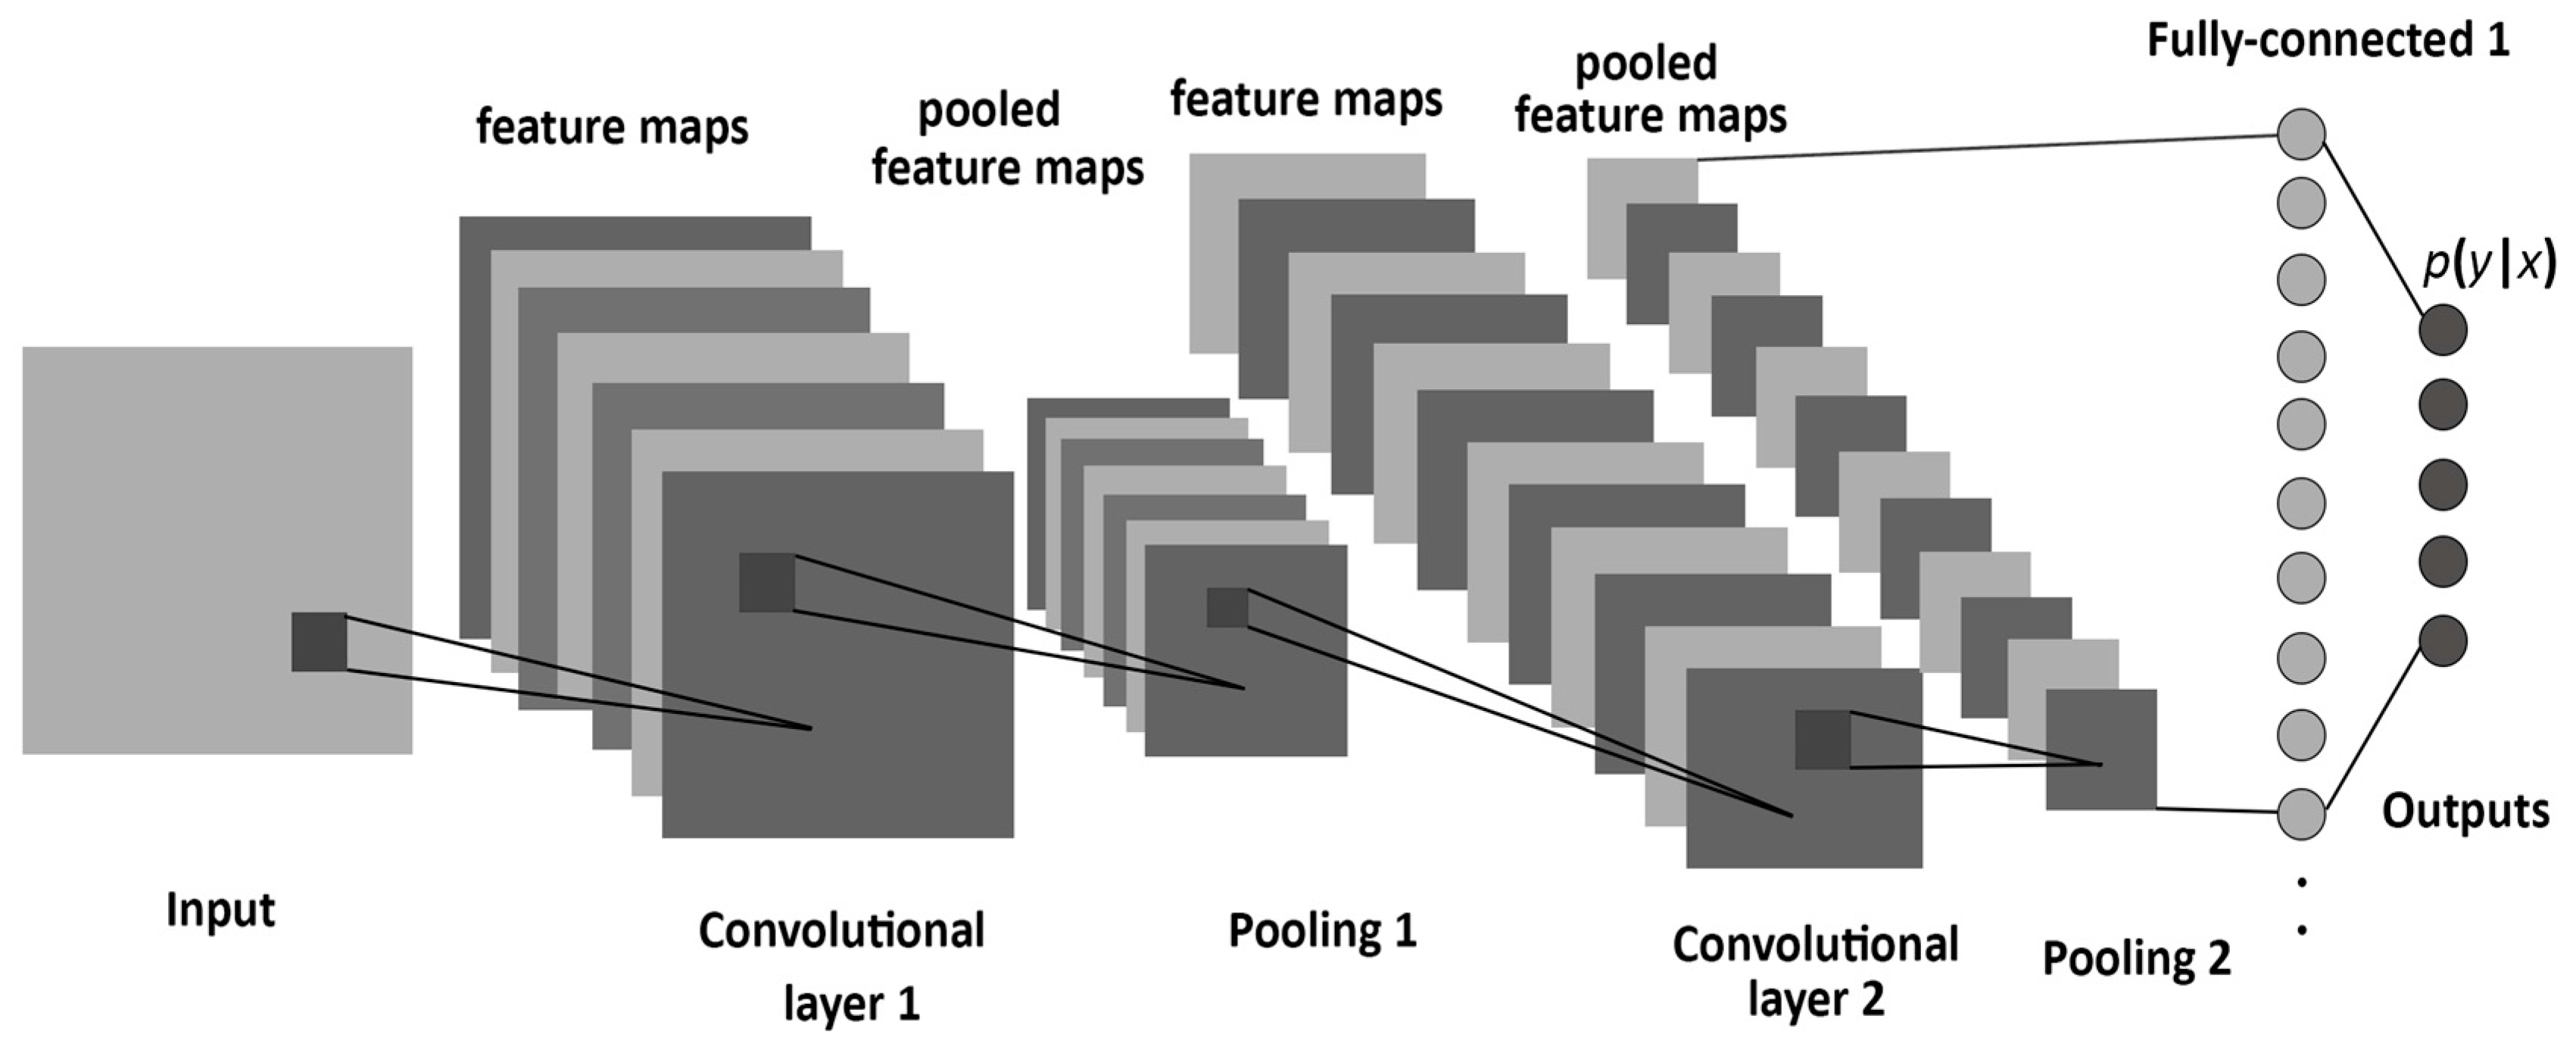
\includegraphics[width=1\textwidth]{img/conv_pooling.png}\\
\caption{A convolutional layer preserves the dimensions of its input matrix, but produces an output with a larger depth dimensions depending on the number of filters. This is followed by pooling layers, which down-sample the data in the width and height dimensions. Image courtesy of  \cite{albelwi2017framework}.}
\label{figure:conv_pooling}
\end{figure}


\subsection{Recurrent Neural Networks}
\textbf{Recurrent neural networks} are a category of neural networks specialized to the processing of data that is temporally sequential. In general, RNNs operate on a sequence of vectors $\bm{x}^{(t)}$, where $t$ is a temporal index into the sequence ranging from $1$ to $T$ \cite[p. 368]{goodfellow2016deep}.

An important concept is that of \textbf{unfolding} a recurrence. For example, the classical equation for dynamic systems
\begin{gather}\label{eq:dynamic_system}
\bm{s}^{(t)} = f_{\bm{\theta}}(\bm{s}^{(t - 1)})
\end{gather}
where $\bm{s}$ is the state of the system, can be unfolded for a finite $t$ by applying the definition $t$ times, removing the recurrence \cite[p. 369-370]{goodfellow2016deep}:
\begin{gather}\label{eq:dynamic_system}
\bm{s}^{(3)} = f_{\bm{\theta}}(f_{\bm{\theta}}(\bm{s}^{(1)}))
\end{gather}

\begin{figure}
\centering
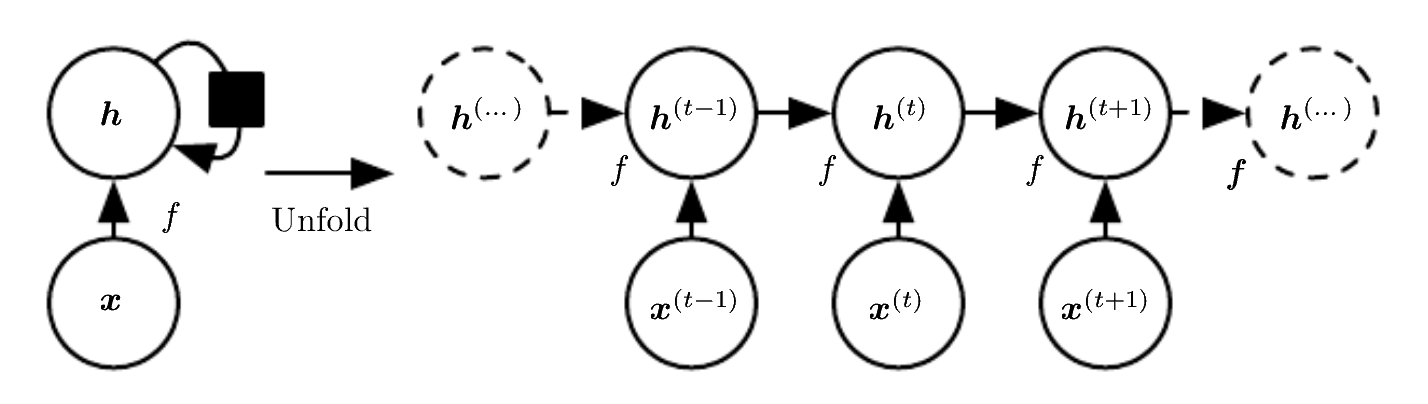
\includegraphics[width=0.7\textwidth]{img/unfolding.png}\\
\caption{Unfolding a recurrent network without outputs. The black square represents a delay of one timestep in the application of previous inputs to the computation. Image courtesy of  \cite[p. 370]{goodfellow2016deep}.}
\label{figure:conv_pooling}
\end{figure}

The behavior of recurrent neural networks is defined by the equation
\begin{gather}\label{eq:recurrent_net}
\bm{h}^{(t)} = f_{\bm{\theta}}(\bm{h}^{(t - 1)}, \bm{x}^{(t)})
\end{gather}

where $\bm{h}$ represents the state of the network, and $\bm{x}$ represents an input to the network. The state of the network is thus dependent on the previous state as well as the current input, and, by induction, on the previous inputs. Goodfellow et al state that "the network typically learns to use $\bm{h}^{(t)}$ as a kind of lossy summary of the task-relevant aspects of the past sequence of inputs up to $t$"\cite{goodfellow2016deep}.

A thorough discussion of recurrent neural networks is beyond the scope of this investigation. Suffice to say that there are many different ways of constructing recurrent neural networks, and typical RNNs include architectural features not captured by equation \ref{eq:recurrent_net}. Similarly to how feed-forward networks can represent almost any function, recurrent neural networks can represent almost any function involving recurrence \cite[p. 370]{goodfellow2016deep}.

According to Goodfellow et al, as of 2016 the most successful type of RNN for practical applications is \textbf{gated RNNs}. This includes \textbf{long short-term memory} (LSTM) networks, which are the type of RNN used in this investigation. The architectural features of LSTM networks enable them to effectively learn long-term dependencies in the temporal input data \cite[p. 404-407]{goodfellow2016deep}.



\subsection{Generative Adversarial Networks}\label{subsection:generativeadversarial}
We may classify machine learning models as either being \textit{discriminative} or \textit{generative}. Examples of discriminative models are neural networks that map images to class labels \cite[p. 1]{goodfellow2014generative}. Generative models, on the other hand, rather than mapping inputs from a training set to class labels, learn to mimic the training set. That is, for a training set of data points drawn from a distribution $p_{data}$, a generative model learns to represent $p_{model}$, an approximation of $p_{data}$ \cite{goodfellow2016nips}.

Goodfellow et al introduced \textbf{generative adversarial networks} (GANs) in 2014, succinctly defining them as a "framework for estimating generative models via an adversarial process", where a discriminative model is used to train a generative model by scrutinizing its outputs \cite{goodfellow2014generative}.

\begin{definition}
A generative adversarial network (GAN) consists of two artificial neural networks, a \textbf{generator} $G$ and a \textbf{discriminator} $D$. The generator represents a function $G_{\theta_{g}}(\bm{z})$ parameterized by weights $\theta_g$, which maps inputs drawn from a distribution $p(\bm{z})$ to outputs in the sample space of $p_{model}(\bm{x})$. The discriminator represents a function $D_{\theta_d}(\bm{x})$ that outputs a single scalar representing the probability that $\bm{x}$ came from the original distribution rather than the generator.

The discriminator is trained to maximize the probability of assigning correct label to both training examples and samples from the generator. In turn, the generator is trained to minimize $\log{1 - D(G(\bm{z}))}$. Goodfellow et all \cite[p. 3]{goodfellow2014generative} showed that this is equivalent to saying that, during training, $D$ and $G$ engage in a two-player minimax game with value function $V(G, D)$, formulated as follows:

\begin{gather}\label{eq:gan_train}
\min_G{\max_D{V(G, D)}} = \mathbb{E}_{\bm{x}~p_{data}(\bm{x})}[\log{D(\bm{x})}] + \mathbb{E}_{\bm{z}~p_{\bm{z}}(\bm{z})}[\log{1 - D(G(\bm{z}))}]
\end{gather}
\end{definition}

A mini-batch stochastic gradient descent training algorithm for a GAN, as given by Goodfellow et al but in simplified form, is shown below.


\begin{minted}{python}
    for i in range(training_iterations):
      for k in range(steps):
        sample mini-batch of samples from data distribution
        sample mini-batch of examples from generator
        updated discriminator by gradient descent
      sample mini-batch of noise from noise distribution
      update generator by gradient descent
\end{minted}

Goodfellow et all also showed that, provided $G$ and $D$ have sufficient capacity, and at each step of the above algorithm $D$ is allowed to reach its optimum given the current $G$, and the generator's weights are updated to decrease the discriminator's performance, then $p_{model}$ converges to $p_{data}$ \cite[p. 5]{goodfellow2014generative}.



\section{Related Work}\label{section:related_work}
Literature review found that few efforts have been made to train neural networks to act as pseudo-random number generators. Research on this topic has garnered very little attention, most likely due to the lack of promising results. In this section, we review the findings of some key papers relevant to this project. The first to be considered, \textit{Learning to Protect Communications with Adversarial Neural Cryptography} provided the inspiration and impetus behind this work.



\subsection{Learning to Protect Communications with Adversarial Neural Cryptography}
The 2016 paper by Google Brain researches Martin Abadi and David Andersen investigates the ability of neural networks in a multiagent environment to learn some form of symmetric-key encryption scheme, enabling some agents to communicate securely. The paper's abstract states:

\say{We ask whether neural networks can learn to use secret keys to protect information from other neural networks. Specifically, we focus on ensuring confidentiality properties in a multiagent system, and we specify those properties in terms of an adversary. Thus, a system may consist of neural networks named Alice and Bob, and we aim to limit what a third neural network named Eve learns from eavesdropping on the communication between Alice and Bob. We do not prescribe specific cryptographic algorithms to these neural networks; instead, we train end-to-end, adversarially. We demonstrate that the neural networks can learn how to perform forms of encryption and decryption, and also how to apply these operations selectively in order to meet confidentiality goals.} \cite{abadi2016learning}

The paper's conclusion mentions pseudo-random number generation as a possible avenue of further investigation, giving origin to this work. 



\subsection{Papers on Using Neural Networks as Pseudo-Random Number Generators}
Overall, literature review carried out for this investigation showed that little research has been carried out on the subject of using neural networks as pseudo-random number generators. A small number of such papers was identified, but all were relatively obscure and presented rather poor results.

For example, a 2012 paper by Veena Desai et al from the Gogte Institute of Technology, \textit{Pseudo random number generator using time delay neural network}, failed to produce a viable neural network-based PRNG, and identified the computational complexity of training networks with thousands of neurons as one of the key challenges \cite{desai2012pseudo}.

Other publications include Desai's earlier 2011 paper  the 2010 paper \textit{Pseudo random number generator using Elman neural network}, as well as the 2010 paper \textit{Hopfield Neural Networks as Pseudo-Random Number Generators}, by Ryverson University's Tirdad and Sadeghian. In all cases the conclusions were mixed at best \cite{desai2011pseudo} \cite{tirdad2010hopfield}. Judging on the difficulty to find material on the topic, and for the meager number of citations for the above paper, one may safely argue that work on this subject has not obtained much attention.



\subsection{Fast, Lean, and Accurate: Modeling Password Guessability Using Neural Networks}
This 2016 paper by Carnegie Mellon University researchers William Melicher et al proposes the use of artificial neural networks as a way of modeling the resistance of passwords. The parts of the paper's abstract that are of direct relevance to this investigation are given below:

\say{Human-chosen text passwords [...] are vulnerable to guessing attacks. [...] We propose using artificial neural networks to model text passwords’ resistance to guessing attacks and explore how different architectures and training methods impact neural networks’ guessing effectiveness. We show that neural networks can often guess passwords more effectively than state-of-the-art approaches [...]. We also show that our neural networks can be highly compressed - to as little as hundreds of kilobytes - without substantially worsening guessing effectiveness [...]} \cite{melicher2016fast}.

The paper is of relevance to this investigation due to the similarities between the core machine learning task tackled in both works. In Melicher et al's paper, a neural network is trained to predict the next character in a sequence of characters. The ability to perform this prediction with a better-than-random-chance probability hinges on the assumption there is a correlation between the characters seen so far, and the next character. This correlation exists due to the fact that the characters in human-chosen passwords are not selected randomly.

Analogously, one aspect of this investigation is the ability to predict the next number in a sequence. Under the assumption of true randomness in the number sequence, no predictive model should be able to perform better than random chance over a sufficiently large number of trials. However, given that each value in the sequence is not \textit{statistically} independent of all other values, this investigation conjectures that a neural network should be capable of learning to predict such a value. The results presented in the paper by Melicher et al arguably supports this conjecture, and informed some architectural design choices for the neural networks involved in this research.





%----------------------------------------------------------
% DESIGN AND IMPLEMENTATION
%----------------------------------------------------------
\chapter{Design and Implementation}\label{chapter:design}
This section provides an in-depth explanation of the conceptual design of the system and how it relates to the research hypothesis, the technologies used to implement it, and the details of the implementation.

\section{Conceptual Design}\label{section:conceptual_design}
As stated, the aim of this investigation is to determine whether it is possible to train a neural network to output pseudo-random number sequences by means of an adversarial training process involving two neural networks, a generator $G$ and an adversary $D$. The goal of this process is to enable the generator to learn a function $G(s, S) : \mathbb{R}^2 \rightarrow \mathbb{R}^n$ which approximates some arbitrary function $prng(s, S) : \mathbb{R}^2 \rightarrow \mathbb{R}^n$, where $prng$ is a function whose outputs fulfill a set of criteria for randomness (subsection \ref{subsection:eval_and_randomness}).

Two distinct approaches are considered. These approaches are termed the \textit{discriminative approach} and the \textit{predictive approach}, and differ in the task performed by the generator's adversary.



\subsection{Generative Model}
The generator, \mintinline{python}{jerry}, implements the function $G_{\theta_{G}}(s, o) : \mathbb{R}^2 \rightarrow \mathbb{R}^n$, where $\theta_G$ are the parameters of $G$, $s$ is the seed of the generator, $o$ is an offset into the generator's output sequence, and $n$ is the length of the output sequence.


\begin{figure}
\centering
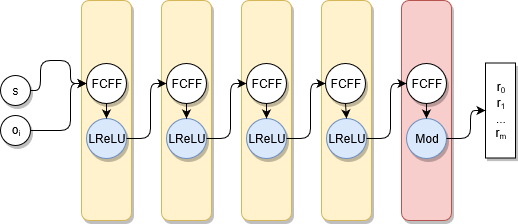
\includegraphics[width=1\textwidth]{img/generator.png}\\
\caption{Architecture of the generator. Each fully connected feed-forward (FCFF) neural network layer is implemented in Keras using a \mintinline{python}{Dense} layer followed by a \mintinline{python}{LeakyReLU} layer. The network's inputs (two real numbers) and outputs (a sequence of real numbers of length $n$) are also shown. Image produced using draw.io \cite{jgraph2018draw}.}
\label{figure:architecture_generator}
\end{figure}

\subsection{Discriminative and Predictive Models}
TODO: architecture of opponents, split into three

\begin{figure}
\centering
\includegraphics[width=1\textwidth]{img/opponent_conv.png}\\
\caption{Convolutional opponent architecture. \mintinline{python}{Reshape} and \mintinline{python}{Flatten} layers are required in Keras as the \mintinline{python}{Conv1D} takes a two-dimensional input. Image produced using draw.io \cite{jgraph2018draw}.}
\label{figure:architecture_conv}
\end{figure}




\subsection{Evaluation and Randomness Requirements}\label{subsection:eval_and_randomness}
The randomness requirements of a cryptographically secure pseudo-random number generator, as well as techniques for assessing whether a potential CSPRNG fulfills them, were discussed in subsections \ref{subsection:crypto_requirements} and \ref{subsection:testing_prngs}, respectively.





\section{Implementation Technologies}
The system was developed using version 3.6 of the Python programming language, which is popular in the machine learning field due to its conciseness and the large ecosystem of software libraries for numerical computing \cite{numpy}. In addition to NumPy, which is ubiquitous in numerical computation using Python \cite{numpy}, the main software librariy used for this project is TensorFlow. The latter is an ``open source library for numerical computation" released by Google, which is commonly used for machine learning \cite{tensorflow}. Most of the code in the implementation deals with abstractions defined in the TensorFlow API.

While Python and the TensorFlow library are popular in the machine learning community, alternatives abound. Programming languages considered for the project included Java and C++, both of which have popular deep learning libraries. Furthermore, TensorFlow is not the only machine learning library available for Python: viable options include Theano, PyTorch, CNTK, and scikit-learn.

Choosing a language, a software library, or a software framework for a particular task is not always straightforward. In this case, Python and TensorFlow were selected due to Python's legibility and simplicity, which supports rapid prototyping, as well as TensorFlow's popularity in the machine learning field, which ensures the availability of abundant documentation, tutorials, and more \cite{bhatia2017why}. The use of these particular technologies is not a critical aspect of this research.

Development of the project was carried out using a mix of free as well as proprietary tools, including the Jetbrains PyCharm integrated development environment and Microsoft's free code editor VSCode. Early tests of the implementation's performance were executed on virtual machines in Google's, Amazon's, and Digital Ocean's cloud services, with a mix of CPU-focused and GPU-focused instance types.

Training of the model was carried out on an HPC cluster, access to which was provided by the School of Electronic Engineering and Computer Science at Queen Mary University of London. The cluster consists of 5 machines, each with 64 CPU cores, 256 GB RAM, and no GPUs.


\subsection{Introduction to TensorFlow}
An introductory guide to the central concepts and functionality of TensorFlow is provided on the software library's website \cite{tensorflow2018intro}. The TensorFlow version used in this project is 1.6.

The central concept is that of the \textit{tensor}, an $n$-dimensional generalization of vectors and matrices. Tensors have properties such as \textit{rank} and \textit{shape}, which specify the number of dimensions of a tensor as well as its size in each dimension \cite{tensorflow2018intro}. TensorFlow programs perform a series of operations on tensors.

At the highest level of abstraction, a TensorFlow program consists of a \textit{Computational Graph} and a \textit{Session}. The former is a directed graph consisting of tensor operations applied to a set of inputs, and defines the topology of a machine learning model. The operations specified in the graph are not computed by the Python interpreter, but rather are first compiled and then executed in TensorFlow's C++ runtime. The Python application interface to the runtime is defined by a TensorFlow Session \cite{tensorflow2018graphs}. When interacting with a session, the act of passing specific inputs to a model for a particular session is referred to as \textit{feeding}, while retrieving the value of a tensor in the graph at a particular time during execution is referred to as \textit{fetching} \cite{tensorflow2018intro}.

The package \mintinline{python}{tf.contrib.gan} in TensorFlow's Python API enables the programmer to easily define generative adversarial networks.


\section{Software Design}
This section outlines the design and implementation of the actual software. The design broadly follows the examples shown by Robin Ricard \cite{ricard2017generative} and Rowel Atienza \cite{atienza2017gan}, and implement the concepts explained in section \ref{section:conceptual_design}.



\subsection{Generative Model}
The generator $G$, known in the code as \mintinline{python}{jerry} or \mintinline{python}{janice}, has the same implementation for both the discriminative and predictive approaches. The model's architecture is defined in TensorFlow as follows:

\begin{minted}{python}
input_layer = tf.reshape(noise, [-1, 2])
outputs = fully_connected(input_layer, GEN_WIDTH, activation=leaky_relu)
outputs = fully_connected(outputs, GEN_WIDTH, activation=leaky_relu)
outputs = fully_connected(outputs, GEN_WIDTH, activation=leaky_relu)
outputs = fully_connected(outputs, GEN_WIDTH, activation=leaky_relu)
outputs = fully_connected(outputs, OUTPUT_SIZE, activation=modulo(MAX_VAL))
return outputs
\end{minted} 

\mintinline{python}{GEN_WIDTH} parameterizes the number of units in each layer. The \mintinline{python}{reshape} operation is used to cast input tensors to an appropriate size. The second argument specifies the shape to which input tensors are cast, where the first value is the tensor's size in the \textit{batch dimension}, and any following values represent the dimensionality of the input samples. The batch dimension refers to the number of input samples in a single batch. In TensorFlow \mintinline{python}{-1} is a special flag signifying dynamic batch size, which allows the model to process its inputs in batches of any size, rather than a fixed size.

The last fully connected layer's \mintinline{python}{modulo} activation function is detailed in subsection \ref{subsection:custom_ops}.


\subsection{Discriminative and Predictive Models}
The discriminator $D$, \mintinline{python}{diego}, and the predictor $P$, \mintinline{python}{priya}, share the same architecture with the exception of the width of the input layer (\mintinline{python}{OUTPUT_SIZE} for \mintinline{python}{diego}, \mintinline{python}{OUTPUT_SIZE - 1} for \mintinline{python}{priya}). This is explained in section \ref{section:conceptual_design}.

The convolutional architecture of the adversaries is implemented as follows:

\begin{minted}{python}
input_layer = tf.reshape(inputs, [-1, size])
outputs = tf.expand_dims(input_layer, 2)
outputs = conv1d(outputs, filters=4, kernel_size=2, strides=1, 
                 padding='same', activation=leaky_relu)
outputs = conv1d(outputs, filters=4, kernel_size=2, strides=1, 
                 padding='same', activation=leaky_relu)
outputs = conv1d(outputs, filters=4, kernel_size=2, strides=1, 
                 padding='same', activation=leaky_relu)
outputs = conv1d(outputs, filters=4, kernel_size=2, strides=1, 
                 padding='same', activation=leaky_relu)
outputs = max_pooling1d(outputs, pool_size=2, strides=1)
outputs = flatten(outputs)
outputs = fully_connected(outputs, 4, activation=leaky_relu)
outputs = fully_connected(outputs, 1, activation=leaky_relu)
return outputs
\end{minted}

The operations \mintinline{python}{flatten} and \mintinline{python}{reshape} are used to modify the shape of tensors in order to connect layers with different shapes. Unlike the generator, where a custom activation function is used in order to introduce more non-linearity, all layers in the adversary model use the popular leaky rectified linear unit activation.



\subsection{Connecting the Models Adversarially}
Keras allows entire models to be treated as layers, and thus models can be composed of other models. Having defined the generator and discriminator/predictor models, they can be combined into a single model.

\begin{minted}{python}
    # define the connected GAN
    discgan_output = jerry(jerry_input)
    discgan_output = diego(discgan_output)
    discgan = Model(jerry_input, discgan_output)
\end{minted}

In this model, the input layer is \mintinline{python}{jerry_input}, i.e. the generator's input layer. The model's stack of layers consists of the generator followed by the discriminator. Crucially, the generator and discriminator are still individually utilizable, but can also be operated on together.

\subsection{Obtaining Training Data}
TODO: how the utility functions work and how the training data is structured
\subsection{Training Procedure for the Discriminative GAN}
TODO: the training procedure
\subsection{Training Procedure for the Predictive GAN}
TODO: the training procedure
\subsection{Custom Tensor Operations}\label{subsection:custom_ops}
The \mintinline{python}{models} package contains modules implementing functionality that is not a part of the TensorFlow API, including custom activation functions and tensor operations. A few notable examples are highlighted here.

\mintinline{python}{drop_last_value(original_size, batch_size)} is a closure returning a callable function \mintinline{python}{layer(x: tf.Tensor)}, which in turn can be used as part of TensorFlow's computational graph. The function defines an operation which drops the last value in a tensor's second dimension, and is used to connect the generator's output layer to the predictor's input layer in the predictive GAN.

\mintinline{python}{modulo(divisor, withActivation=None)} is a closure returning a custom activation function that computes the modulus $\mod{divisor}$ of its input. It is also possible to use it in conjunction with another activation function, which can be passed to the second parameter.


\subsection{Utilities}
A number of utility modules are defined to abstract the details of auxiliary procedures, such as logging, producing plots of training results, or generating samples of pseudo-random numbers for training the neural networks. An overview of the role of each utility module within the system is given below. A more detailed view of the functionality of these modules can be obtained from the source code and its documentation.

The \mintinline{python}{utils.input_utils.py} module defines functions for the \textbf{generation of training data}. Provided functionality includes generation of a single real-valued pseudo-random scalar, of a one-dimensional list of such scalars, or of matrices of inputs suitable for supervised training of either network in the adversarial models.

The \mintinline[breaklines]{python}{utils.operation_utils.py} module provides \textbf{common operations on tensors or Numpy arrays}. These include element-wise logarithms on tensors in an arbitrary base, flattening multidimensional lists with irregular internal structure, splitting the output of the generator into an $(input, label)$ pair for training the predictor, and setting the trainability of parameters in Keras model.

The \mintinline{python}{utils.vis_utils.py} module handles the creation and storage of \textbf{graphical visualizations}. This includes primarily drawing plots of training loss or histograms of output distributions, as well as graphs of neural network structures.

The remaining modules provide miscellaneous functionality such as error printing and logging information to text files.


%----------------------------------------------------------
% EXPERIMENTS
%----------------------------------------------------------
\chapter{Experiments}\label{chapter:experiments}
This section outlines the training and evaluation procedure followed in order to test this work's hypothesis. A large number of "throwaway" tests was performed over an extended period of time to empirically identify good training setups, ranging from parameters such as learning rate to major design choices in neural network architecture. Finally, the models were trained multiple times in order to produce output samples, which were evaluated using the dieharder test suite.


\section{Training and Evaluation Procedure}
The general experimental procedure entails adversarially training the generator and the opponent for a fixed number of iterations, and producing a text file of output samples from the generator, both before training and when training is complete. These text files are analyzed by dieharder in order to assess whether training improved the generator's performance in the statistical randomness tests.



- alternating training in general
- first pretrain ( ON WHAT DATA
- then main train (ON WHAT DATA)
- evaluate periodically (HOW, ON WHAT DATA)
- final evaluation

\section{Training and Evaluation Parameters}


\section{Neural Network Hyperparameters}
The learning algorithm's hyperparameters were selected by running a number of shorter tests, in order to identify how different hyperparameters affected the performance of the model. This process relied entirely on the author's intuition and exploratory testing. Automated hyperparameter optimization was not performed.

Some of the most significant hyperparameters include the networks' learning rate and their degree of decay, the generator width, the adversary width, the input batch size, and the generator output size. Their values, and the heuristics by which they were chosen, are given below.

\begin{enumerate}
\item \mintinline{python}{LEARNING_RATE: 0.02} - 
\item \mintinline{python}{OPTIMIZER_DECAY_ALPHA: 0.999} - 
\item \mintinline{python}{OPTIMIZER_DECAY_BETA: 0.999} - 
\item \mintinline{python}{GEN_WIDTH: 30} - 
\item \mintinline{python}{CONV_WIDTH} - 
\item \mintinline{python}{} - 
\item \mintinline{python}{} - 
\end{enumerate}


A number of other hyperparameters, in particular those parameterizing the convolutional layers, are not considered here.


\section{Results}


%----------------------------------------------------------
% CONCLUSION
%----------------------------------------------------------
\chapter{Conclusion}\label{chapter:conclusion}
TODO: if generator works, conclude that work backs the conjecture that a discrete uniform distribution can be learned by a neural network. If it doesn't, conclusion should state why. In either case probably more experimentation is required as these experiments were constrained due to a number of reasons.


%----------------------------------------------------------
% FURTHER INVESTIGATION
%----------------------------------------------------------
\chapter{Further Investigation}
TODO: more formal treatment of the problem, such as cryptanalysis if the generator works, or an in-depth analysis of failure if it doesn't. Further attempts with better training procedure, i.e. hyperparameter optimization, cross-validation of architectures, etc? There are quite many training improvements that could be implemented, list them.


%--------------------------------------------------
% BIBLIOGRAPHY
%--------------------------------------------------
\bibliographystyle{plain}
\bibliography{references.bib}


%----------------------------------------------------------
% APPENDICES
%----------------------------------------------------------
\appendix
\chapter{Training Data}
TODO: currently being trained as of draft submission. Data will be outputted to files so can easily be extracted, tabled, graphed, etc.

\chapter{Code Listings}
\section{Generator}\label{appendix:generator}
\begin{minted}{python}
    inputs = Input(shape=(2,))
    outputs = Dense(GEN_WIDTH)(inputs)
    outputs = LeakyReLU(ALPHA)(outputs)
    outputs = Dense(GEN_WIDTH)(outputs)
    outputs = LeakyReLU(ALPHA)(outputs)
    outputs = Dense(GEN_WIDTH)(outputs)
    outputs = LeakyReLU(ALPHA)(outputs)
    outputs = Dense(GEN_WIDTH)(outputs)
    outputs = LeakyReLU(ALPHA)(outputs)
    outputs = Dense(OUTPUT_SIZE)(outputs)
    outputs = LeakyReLU(ALPHA)(outputs)
    generator = Model(inputs, outputs, name=name)
\end{minted} 

\section{Adversary, Convolutional Architecture}\label{appendix:convolutional}
\begin{minted}{python}
    inputs = Input((input_size,))
    outputs = Reshape(target_shape=(input_size, 1))(inputs)
    outputs = Conv1D(filters=2, kernel_size=2, strides=1, padding='same')(outputs)
    outputs = LeakyReLU(ALPHA)(outputs)
    outputs = Conv1D(filters=2, kernel_size=2, strides=1, padding='same')(outputs)
    outputs = LeakyReLU(ALPHA)(outputs)
    outputs = MaxPooling1D(2)(outputs)
    outputs = Conv1D(filters=4, kernel_size=2, strides=1, padding='same')(outputs)
    outputs = LeakyReLU(ALPHA)(outputs)
    outputs = Conv1D(filters=4, kernel_size=2, strides=1, padding='same')(outputs)
    outputs = LeakyReLU(ALPHA)(outputs)
    outputs = MaxPooling1D(2)(outputs)
    outputs = Flatten()(outputs)
    outputs = Dense(2)(outputs)
    outputs = LeakyReLU(ALPHA)(outputs)
    outputs = Dense(1)(outputs)
    outputs = LeakyReLU(ALPHA)(outputs)
    discriminator = Model(inputs, outputs)
\end{minted}

\section{Adversary, LSTM Architecture}\label{appendix:lstm}
\begin{minted}{python}
    inputs = Input((input_size,))
    outputs = Reshape(target_shape=(input_size, 1))(inputs)
    outputs = LSTM(1, return_sequences=True)(outputs)
    outputs = LeakyReLU(ALPHA)(outputs)
    outputs = LSTM(1, return_sequences=True)(outputs)
    outputs = LeakyReLU(ALPHA)(outputs)
    outputs = LSTM(1, return_sequences=True)(outputs)
    outputs = LeakyReLU(ALPHA)(outputs)
    outputs = Flatten()(outputs)
    outputs = Dense(int(input_size / 2))(outputs)
    outputs = LeakyReLU(ALPHA)(outputs)
    outputs = Dense(2)(outputs)
    outputs = LeakyReLU(ALPHA)(outputs)
    outputs = Dense(1)(outputs)
    outputs = LeakyReLU(ALPHA)(outputs)
    discriminator = Model(inputs, outputs)
    discriminator.compile(optimizer, loss)
\end{minted}

\section{Adversary, Convolutional LSTM Architecture}\label{appendix:convlstm}
\begin{minted}{python}
    inputs = Input((input_size,))
    outputs = Reshape(target_shape=(input_size, 1))(inputs)
    outputs = Conv1D(filters=2, kernel_size=2, strides=1, padding='same')(outputs)
    outputs = LeakyReLU(ALPHA)(outputs)
    outputs = Conv1D(filters=2, kernel_size=2, strides=1, padding='same')(outputs)
    outputs = LeakyReLU(ALPHA)(outputs)
    outputs = Flatten()(outputs)
    outputs = Reshape(target_shape=(input_size, 2))(outputs)
    outputs = LSTM(1, return_sequences=True)(outputs)
    outputs = LeakyReLU(ALPHA)(outputs)
    outputs = LSTM(1, return_sequences=True)(outputs)
    outputs = LeakyReLU(ALPHA)(outputs)
    outputs = LSTM(1, return_sequences=True)(outputs)
    outputs = LeakyReLU(ALPHA)(outputs)
    outputs = Flatten()(outputs)
    outputs = Dense(4)(outputs)
    outputs = LeakyReLU(ALPHA)(outputs)
    outputs = Dense(2)(outputs)
    outputs = LeakyReLU(ALPHA)(outputs)
    outputs = Dense(1)(outputs)
    outputs = LeakyReLU(ALPHA)(outputs)
    discriminator = Model(inputs, outputs)
\end{minted}

\section{Training of Discriminative GAN}\label{appendix:training_discgan}
\begin{minted}{python}
 # main training procedure
    jerry_loss, diego_loss = np.zeros(EPOCHS), np.zeros(EPOCHS)
    try:
        for epoch in range(EPOCHS):
            # training data for this epoch
            seeds, offsets, jerry_labels = get_inputs(BATCH_SIZE * BATCHES, MAX_VAL)
            jerry_inputs = np.array([seeds, offsets]).transpose()

            for batch in range(BATCHES):
                # generate batch data
                jerry_x = extract_batch(jerry_inputs, batch, int(BATCH_SIZE / 2))
                jerry_y = extract_batch(jerry_labels, batch, int(BATCH_SIZE / 2))
                diego_x, diego_y = get_sequences(jerry, jerry_x, OUTPUT_SIZE, MAX_VAL)

                # alternate train
                set_trainable(diego, DIEGO_OPT, DIEGO_LOSS, RECOMPILE)
                for i in range(ADV_MULT):
                    diego_loss[epoch] += diego.train_on_batch(diego_x, diego_y)
                set_trainable(diego, DIEGO_OPT, DIEGO_LOSS, RECOMPILE, False)
                jerry_loss[epoch] += discgan.train_on_batch(jerry_x, jerry_y)

            # log debug info to console
            diego_loss[epoch] /= (BATCHES * ADV_MULT)
            jerry_loss[epoch] /= BATCHES
            if not HPC_TRAIN or epoch % LOG_EVERY_N == 0:
                print_epoch(epoch, gen_loss=jerry_loss[epoch], opp_loss=diego_loss[epoch])
            # check for NaNs
            if math.isnan(jerry_loss[epoch]) or math.isnan(diego_loss[epoch]):
                raise ValueError()

    except ValueError:
        traceback.print_exc()
\end{minted}

\section{Training of Predictive GAN}\label{appendix:training_predgan}
\begin{minted}{python}
    # main training procedure
    janice_loss, priya_loss = np.zeros(EPOCHS), np.zeros(EPOCHS)
    try:
      for epoch in range(EPOCHS):
        # get data for this epoch
        janice_inputs = np.array(get_inputs(BATCH_SIZE * BATCHES, MAX_VAL)[:-1]).transpose()

        for batch in range(BATCHES):
          # generate predictions for this batch
          janice_x = extract_batch(janice_inputs, batch, BATCH_SIZE)
          priya_x, priya_y = detach_all_last(janice.predict_on_batch(janice_x))

          # train both networks on entire dataset
          set_trainable(priya, PRIYA_OPT, PRIYA_LOSS, RECOMPILE)
            for i in range(ADV_MULT):
              priya_loss[epoch] += priya.train_on_batch(priya_x, priya_y)
            set_trainable(priya, PRIYA_OPT, PRIYA_LOSS, RECOMPILE, False)
            janice_loss[epoch] += predgan.train_on_batch(janice_x, priya_y)

        # update and log loss value
        priya_loss[epoch] /= (BATCHES * ADV_MULT)
        janice_loss[epoch] /= BATCHES
        if epoch % LOG_EVERY_N == 0:
          print_epoch(epoch, gen_loss=janice_loss[epoch], opp_loss=priya_loss[epoch])
        # check for NaNs
        if math.isnan(janice_loss[epoch]) or math.isnan(priya_loss[epoch]):
          raise ValueError()

    except ValueError:
        traceback.print_exc()
\end{minted}

\chapter{Mathematical Notation}\label{appendix:mathematics}
The mathematical notation used in this work is outlined in this appendix. The notation followed is primarily drawn from the seminal computer science textbook \textit{Introduction to Algorithms}, by Cormen, Leiserson, Rivest, and Stein \cite{cormen2009introduction}. Unless otherwise stated, all definitions in this appendix should be assumed to be verbatim from this source, preserving the precision of the language of the source. Quotation marks and statements such as ``according to Cormen, Leiserson, Rivest, and Stein ..." shall be implicit.

\section{Set Theory}
TODO: fill in 
\section{Probability Theory}
\textbf{Definition}. The \textbf{sample space} $\Omega = \{w_1, w_2, ..., w_n\}$ of an experiment is the set of all possible \textbf{outcomes} $w_i$. An \textbf{event} is a subset $A \subset \Omega$ of the sample space. The outcomes may also be referred to as \textbf{elementary events}, in that for every outcome $w_i$, there is an event $A_i = \{w_i\}$.

\textbf{Definition}. A \textbf{probability distribution} $p(\Omega)$ is a function $p : \Omega \rightarrow \mathbb{R}$ satisfying the three \textbf{probability axioms}:
\section{Linear Algebra}
\begin{definition}
The \textbf{convolution} operation
\end{definition}

\section{Neural Networks}
\begin{definition}
The \textbf{sigmoid} activation is a function $\sigma : \mathbb{R} \rightarrow [0, 1]$ with the following expression form:
\begin{gather}\label{eq:sigmoid}
\sigma(x)=1/(1 + {e^{-x}})
\end{gather}

The sigmoid activation function "compresses" its inputs into to the range $[0, 1]$. In particular, the output value approaches $1$ as the input tends to positive infinity, and approaches $0$ as the input tends to negative infinity.
\end{definition}

The sigmoid activation is traditionally one of the most used sources of non-linearity in neural networks. However, it suffers from a few drawbacks. For one, the sigmoid function is detrimental to gradient descent, as the gradient of the sigmoid function is effectively zero for the vast majority of its inputs.

\begin{definition}
The \textbf{tanh} activation is a function $tanh: \mathbb{R} \rightarrow [-1, 1]$ with the following expression form:
\begin{gather}\label{eq:tanh}
tanh(x)=2\sigma(2x)-1
\end{gather}
\end{definition}


\end{document}
